\documentclass{article}\usepackage[]{graphicx}\usepackage[]{color}
% maxwidth is the original width if it is less than linewidth
% otherwise use linewidth (to make sure the graphics do not exceed the margin)
\makeatletter
\def\maxwidth{ %
  \ifdim\Gin@nat@width>\linewidth
    \linewidth
  \else
    \Gin@nat@width
  \fi
}
\makeatother

\definecolor{fgcolor}{rgb}{0.345, 0.345, 0.345}
\newcommand{\hlnum}[1]{\textcolor[rgb]{0.686,0.059,0.569}{#1}}%
\newcommand{\hlstr}[1]{\textcolor[rgb]{0.192,0.494,0.8}{#1}}%
\newcommand{\hlcom}[1]{\textcolor[rgb]{0.678,0.584,0.686}{\textit{#1}}}%
\newcommand{\hlopt}[1]{\textcolor[rgb]{0,0,0}{#1}}%
\newcommand{\hlstd}[1]{\textcolor[rgb]{0.345,0.345,0.345}{#1}}%
\newcommand{\hlkwa}[1]{\textcolor[rgb]{0.161,0.373,0.58}{\textbf{#1}}}%
\newcommand{\hlkwb}[1]{\textcolor[rgb]{0.69,0.353,0.396}{#1}}%
\newcommand{\hlkwc}[1]{\textcolor[rgb]{0.333,0.667,0.333}{#1}}%
\newcommand{\hlkwd}[1]{\textcolor[rgb]{0.737,0.353,0.396}{\textbf{#1}}}%
\let\hlipl\hlkwb

\usepackage{framed}
\makeatletter
\newenvironment{kframe}{%
 \def\at@end@of@kframe{}%
 \ifinner\ifhmode%
  \def\at@end@of@kframe{\end{minipage}}%
  \begin{minipage}{\columnwidth}%
 \fi\fi%
 \def\FrameCommand##1{\hskip\@totalleftmargin \hskip-\fboxsep
 \colorbox{shadecolor}{##1}\hskip-\fboxsep
     % There is no \\@totalrightmargin, so:
     \hskip-\linewidth \hskip-\@totalleftmargin \hskip\columnwidth}%
 \MakeFramed {\advance\hsize-\width
   \@totalleftmargin\z@ \linewidth\hsize
   \@setminipage}}%
 {\par\unskip\endMakeFramed%
 \at@end@of@kframe}
\makeatother

\definecolor{shadecolor}{rgb}{.97, .97, .97}
\definecolor{messagecolor}{rgb}{0, 0, 0}
\definecolor{warningcolor}{rgb}{1, 0, 1}
\definecolor{errorcolor}{rgb}{1, 0, 0}
\newenvironment{knitrout}{}{} % an empty environment to be redefined in TeX

\usepackage{alltt}
\title{\vspace{-1cm}}
\author{\textbf{Midterm Examination} \\ \textbf{Katherine Wolf} \\ PH250C Spring 2020 \\ March 31, 2020}
\date{}

% list of latex packages you'll need
\usepackage{float}  % for tables
\usepackage{mathtools}  % for mathematical symbols
\usepackage{bm}  % to bold mathematical symbols like betas
\usepackage{scrextend}  % to indent subsections
\usepackage{xltxtra}
\usepackage{fontspec}
\usepackage{xunicode}
\usepackage[skip=0.5\baselineskip]{caption}  % control caption printing space
\usepackage{longtable}
\usepackage{amsmath}
\usepackage{amsfonts}
\usepackage{bm}
\usepackage{caption}
\usepackage[shortlabels]{enumitem}
\usepackage{txfonts}
\usepackage{dejavu}
\usepackage{mathpazo}

% set fonts
\setmainfont{Palatino Linotype}
\setsansfont{Corbel}
\setmonofont{Consolas}

% set the margins of the document
\usepackage[top=.5in, bottom=.9in, left=.5in, right=.5in]{geometry}

% remove automatic indenting
\setlength{\parindent}{0pt}

% end the preamble and begin the document
\IfFileExists{upquote.sty}{\usepackage{upquote}}{}
\begin{document}

\maketitle

\vspace{-.5cm}

\begin{enumerate}[label=\textbf{\arabic*.}]

  \item \textbf{Background.} Both exposure to fine particulate matter $\leq 2.5$ microns in diameter (PM\textsubscript{2.5}) and racial residential segregation, the separation of two or more groups into different neighborhoods by race, of African Americans in the United States (US) have been associated with common negative health outcomes including cardiovascular disease, respiratory disease, lung cancer, low birthweight, preterm birth, and death. Evidence is mounting that the toxicity of PM\textsubscript{2.5} varies according to its chemical composition. Moreover, component concentrations can be used to identify PM\textsubscript{2.5} sources.
  
  \item \textbf{Specific aim.} We will estimate the association between racial residential segregation and PM\textsubscript{2.5} component concentrations in census tracts in urban areas of the United States.
  \item \textbf{Approach.}
  
  \begin{enumerate}[label=\textbf{\alph*.}]
    
    \item \textbf{Study population.} The population for this study will include the 886 census tracts both (1) classified as urban by Department of Agriculture Rural-Urban Commuting Area codes and (2) that contain Environmental Protection Agency (EPA) Chemical Speciation Network (CSN) monitors with at least 3 years and 180 days of observations from 2005 to 2015.
    
    \item \textbf{Outcome.} The outcomes for this study will be the 2005-2015 ten-year mean concentration in micrograms ($\mu g$) per cubic meter ($m^3$) of PM\textsubscript{2.5} components\footnote{Components include (where $n$ indicates the number of urban census tracts with at least 180 daily observations of that component over at least 3 years) total PM\textsubscript{2.5} ($n=886$), aluminum ($n=276$), arsenic (As) ($n=276$), bromine (Br) ($n=274$), cadmium ($n=276$), calcium ($n=276$), chlorine ($n=276$), copper (Cu) ($n=275$), iron (Fe) ($n=276$), lead (Pb) ($n=276$), mercury ($n=162$), nickel (Ni) ($n=276$), silicon ($n=276$), sodium ($n=264$), titanium ($n=276$), vanadium (V) ($n=276$), zinc (Zn) ($n=276$), ammonium ion (NH4+) ($n=213$), sodium ion ($n=213$), nitrate ion (NO3–) ($n=267$), sulfate ion (SO42–) ($n=277$), and elemental carbon (EC) ($n=201$).} generated by calculating the mean of monthly means of daily means measured by the Environmental Protection Agency Chemical Speciation Network of PM\textsubscript{2.5} component monitors within a census tract.
    
    \textbf{Exposure.} The exposure for this study will be the Black racial isolation in a census tract as measured by the spatial isolation index developed by Anthopolos et al.\footnote{Anthopolos R, James SA, Gelfand AE, Miranda ML. A spatial measure of neighborhood level racial isolation applied to low birthweight, preterm birth, and birthweight in North Carolina. Spat Spatiotemporal Epidemiol 2011;2(4):235–46.}. The index ranges from 0 (no spatial isolation, in which a Black census tract resident only encounters non-Black neighbors) to 1 (complete spatial isolation, in which a Black census tract resident only encounters Black neighbors).
    
    \textbf{Confounders.} Models will consider covariate adjustment for 
\begin{itemize}
  \item Total census tract population (persons)
  \item Population density (persons per square kilometer)
  \item Sex (percent female)
  \item Race/ethnicity, including percent white (not Hispanic or Latinx), Percent Hispanic or Latinx (any race), percent African American (not Hispanic or Latinx), percent Asian (not Hispanic or Latinx), and percent other
  \item Median home value of owner-occupied housing units (dollars)
  \item Median household income (dollars)
  \item Age, including percent 0-19 years old and percent 65 years old and older
  \item Housing tenure (percent of homes renter-occupied)
  \item Linguistic isolation (percent of households in which no one 14 and over either (1) speaks English only or (2) speaks a language other than English at home and speaks English "very well")
  \item Education (percent of adults $\geq$ 25 years of age with less than a high school education)
  \item Poverty (percent of the population in poverty)
  \item Unemployment (percent of households with one family member unemployed)
  \item Region (Midwest, Northeast, South, West)
\end{itemize}
    
    \item \textbf{Target parameter.} We seek to estimate the change in the concentration (in $\mu g/m^3$)) of each PM\textsubscript{2.5} component per 0.2-unit change in African American spatial isolation, holding the values of the other covariates listed above constant. We will use a restricted polynomial spline model to avoid the assumption of a linear dose-response relationship.
    
    \end{enumerate}
  
  \item \textbf{Methodological issue.} One important limitation of the proposed analysis is selection bias induced by the limitation of the study to census tracts containing EPA CSN PM\textsubscript{2.5} component monitors. For example, racism in governmental bodies regulating land uses might affect Black racial isolation in neighbhorhoods (via decisions on acceptable land uses, mortgages, etc.), monitor siting and activity, and the presence of PM\textsubscript{2.5} sources. Meanwhile, the EPA explicitly prioritizes monitoring in areas where they expect to find exceedances of federal PM\textsubscript{2.5} standards, particularly in areas with known PM\textsubscript{2.5} sources that have produced PM\textsubscript{2.5} exceedances in the past. The selection bias results from conditioning (selecting census tracts based) on an effect (presence of an active monitor) of both an unmeasured cause of the exposure (racism in governmental bodies) and an unmeasured cause of the outcome (presence of a PM\textsubscript{2.5} source). (Racism in governmental bodies, by affecting siting decisions for PM2.5 component sources, also induces ordinary unmeasured confounding by opening a backdoor path between the exposure and the outcome that runs exclusively through unmeasured variables in the current study). A simplified directed acyclic graph (DAG) illustrating the problem is shown below in Figure 1.\footnote{Hernán MA, Hernández-Díaz S, Robins JM. A Structural Approach to Selection Bias: Epidemiology 2004;15(5):615–25. doi:10.1097/01.ede.0000135174.63482.43. This particular form of selection bias takes the form of the bias illustrated in Figure 6c on page 617, but with additional ordinary unmeasured confounding introduced by the arrow from "racism in governmental bodies regulating land uses (unmeasured)", which causes the exposure, to "PM\textsubscript{2.5} component source present (unmeasured)", which causes the outcome.}
  
  \textbf{Figure 1. DAG showing selection bias from including only census tracts with PM\textsubscript{2.5} component monitors.}
  
  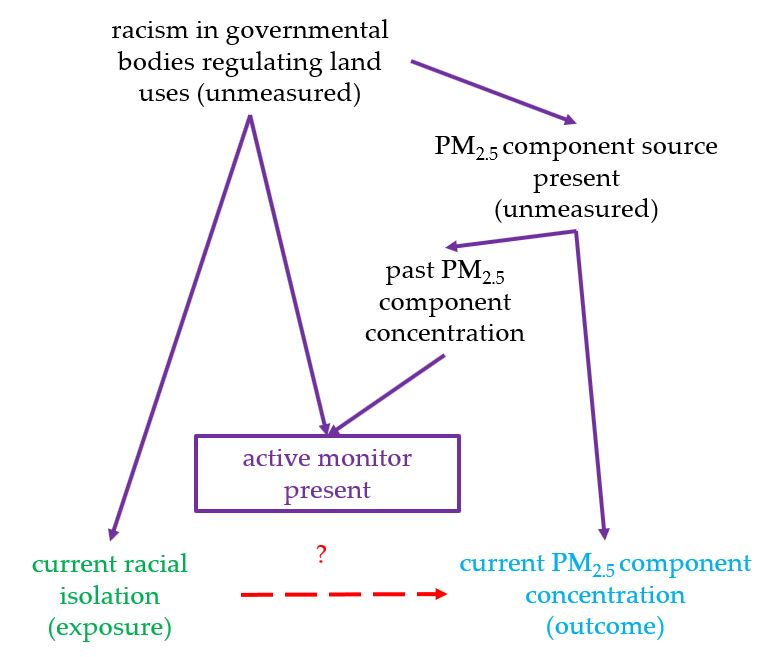
\includegraphics[height=2.3in]{midtermdag.JPG}

Another limitation of the proposed analysis is the missing (but bounded) data in the outcome variables, ten-year mean PM\textsubscript{2.5} component concentrations, due to the relationship between the ambient concentrations of the PM\textsubscript{2.5} components and the monitor method detection limit (MDL) for each component. Figure 1 shows the percentage of observations (daily means) below the MDL for each PM\textsubscript{2.5} component.\footnote{I realize that I am only supposed to identify one, but I add this second one because I would genuinely love advice on how to deal with it.}

  \textbf{Figure 2. Percentage of observations (daily means) below the MDL for each PM\textsubscript{2.5} component.}

  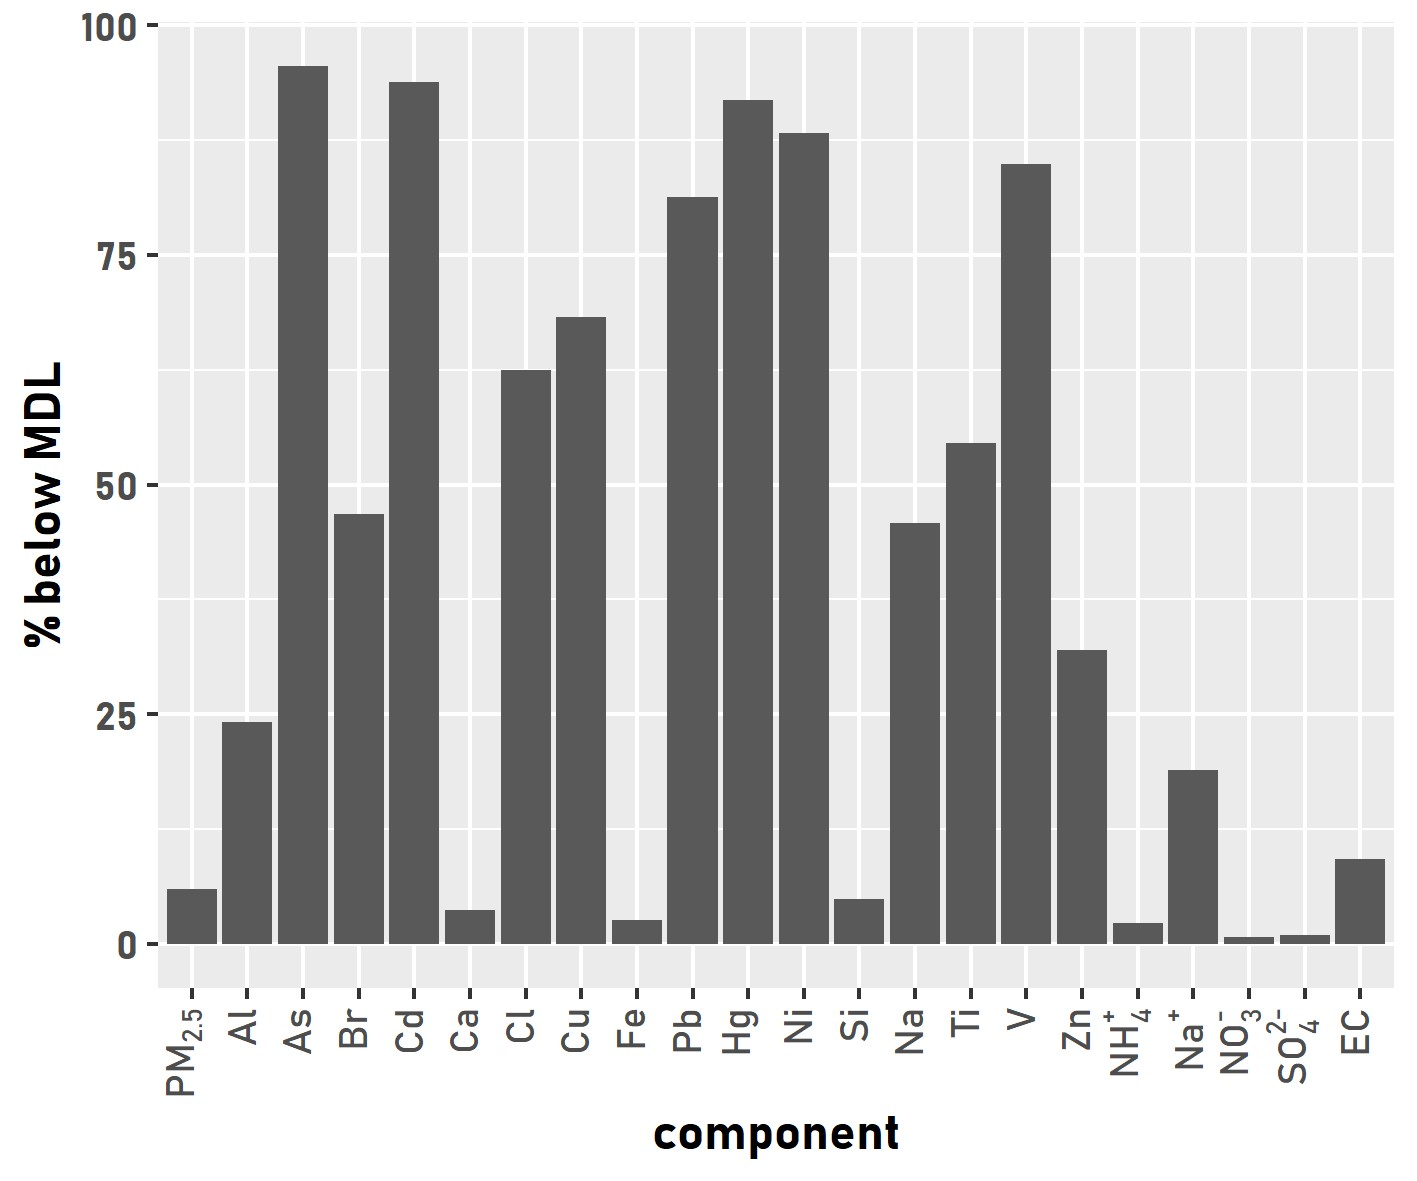
\includegraphics[height=2.3in]{detectionlimit.jpg}

\end{enumerate}
      
\end{document}
